
\chapter{Metric spaces}
\section{Definitions and examples}
%create a math proof environment
	\paragraph{\it Excercise 1.1.1.}{\it Proof.} $\Rightarrow \forall\varepsilon \quad\exists N\quad\text{s.t.} \quad\forall n \geqslant N\quad |x_{n}-x| \leqslant\varepsilon$ which is to say $\diff (x_{n},x) \leqslant \varepsilon$. Therefore, $\lim_{n\rightarrow\infty}\diff(x_{n},x)=0$.\\
	
	$\Leftarrow \quad \forall\varepsilon \quad\exists N\quad\text{s.t.} \quad\forall n \geqslant N\quad \diff(x_{n},x)\leqslant\varepsilon $ which means $ |x_{n}-x| \leqslant\varepsilon$\\Therefore, $(x_{n})_{n=m}^{\infty}$ indeed converges to $x$.

\paragraph{\it Excercise 1.1.2.}

\paragraph{\it Excercise 1.1.3.}
\begin{itemize}
\item[(a)]d(x,y):=0.5(x=y),1(x$\neq$y)
\item[(b)]d(x,y):=0 (for any x,y$\in$X)
\item[(c)]X:=\{x,y,z\}  d(x,y):=0.5; d(y,x):=1;d(a,b):=1 (a$\neq$b).d(a,b):=0(a=b)
\item[(d)]Pick three point on a line makes X. Their distances in between be 1,1,3.

\end{itemize}


\paragraph{Excercise 1.1.4}
Firstly, the subset and restricted function all induced four properties or we say they satisfied four axioms automatically.

\paragraph{Excercise 1.1.5}
First equation use induction.
With the first equation, we can get second equation directly(remove the second part, positive, on the left hand side and then find square root of both sides).(see also linear algebra for a different proof)\\
With a little bit arrange( square the inequality and exchange finite summation symbol), we can get the final inequatlity.
\paragraph{Exercise 1.1.6}
Just get used to four axioms of being a metric space.With the help of third inequality in excercise1.1.5 for forth axiom.
\paragraph{Exercise 1.1.7.}
Nothing special.
\paragraph{Exercise 1.1.8.}Hint on the book said clearly enough.
\paragraph{Exercise 1.1.9.}For (a)(b)(c), there isn't much to say. For (d), d($x$,$z$)=sup\{|$x_{i}$-$z_{i}$|:1$\leqslant$$i$$\leqslant$$n$\}. Let's say $i_{0}$, d($x$,$z$)=|$x_{i_{0}}$-$z_{i_{0}}$|. Then\[ |x_{i_{0}}-z_{i_{0}}|\leqslant|x_{i_{0}}-y_{i_{0}}|+|y_{i_{0}}-z_{i_{0}}|
\]
Which is the same as \[d(x,z)
\leqslant|x_{i_{0}}-y_{i_{0}}|+|y_{i_{0}}-z_{i_{0}}|
\]
Considering the definition of $d(x,y)$,$d(y,z)$, the target inequality holds.
\[d(x,z)
\leqslant d(x,y)+d(y,z)\]
\paragraph{Exercise 1.1.10}
left as excercise---surely I'm joking
Though, it's fairly easy let's write it down.Right hand side really no need to do.\\Left hand side:let $\sup_{i=1}^{n}|x_{i}-y{i}|=|x_{i_{0}}-y_{i_{0}}|$\[\frac{1}{\sqrt{n}}\sqrt{\sum_{i=1}^{n}(x_{i}-y_{i})^2}\leq\sqrt{\frac{\sum_{i=1}^{n}(x_{i_{0}}-y_{i_{0}})^2}{n}}=\sup_{i=1}^{n}|x_{i}-y_{i}|\]
\paragraph{Exercise 1.1.12}
With inequality (1.1), (1.2)in the book, it's trivial to see (a)(b)(c) are equivalent.(why?) \[d_{l^2}(x,y)\leq d_{l^1}(x,y)\leq\sqrt{n}d_{l^2}(x,y) \]%label it\quad(1)
\[\frac{1}{\sqrt{n}}d_{l^2}(x,y)\leq d_{l^\infty}(x,y)\leq d_{l^2}(x,y) \]
The remaining part is just to show (c) and (d) are equivalent.\\
$Proof: $\\$\Rightarrow :$$\forall \varepsilon $ there $\exists K \text{ s.t.}$ $\forall k \geqslant K$, $ d_{l^\infty}(x^{(k)},x)\leq \varepsilon$ \\
Which means $\sup_{k=1}^{n}|x_{i}^{(k)}-x|\leq \varepsilon$;
Certainly implies, for every$1 \leq j \leq n$, the sequence $ {(x_{j}^{(k)})}_{k=m}^{\infty}$ converges.\\$\Leftarrow$For there is only finite m, we can choose a largest $K$ to make (c) come true.
\paragraph{Excercise 1.1.13}$\Leftarrow$ is obvious.\\
$\Rightarrow$ Assume, it isn't the case,$\forall N, \exists m \geq N,\text{ s.t } x_{m}\neq x$ which means $ \forall N, \exists m, \text{ s.t. }\\d(x_{m},x)=1$ Which is contradict to $\lim_{n\rightarrow\infty}d(x_{n},x)=0$ ($x_{n}$ converges to x see excercise 1.1.1.)$\Box$
\paragraph{Exercise 1.1.14}
$\forall \frac{\varepsilon}{3}$, $\exists N$ s.t. when $m, n\geq N$, $d(x_{n},x)\leq\frac{\varepsilon}{3}$, $d(x_{n},x_{m})\leq\frac{\varepsilon}{3}$ (convergence implies Cauchy), $d(x_{m},x^{\prime})\leq\frac{\varepsilon}{3}$\\Then, by four axioms of metric space, we know $d(x^{\prime},x)\leq \varepsilon$ for any $\varepsilon$. Which implies $d(x^{\prime},x)\leq 0$. By axiom (a), $d(x^{\prime},x)=0$. By (c), $x=x^{\prime}$.$\Box$

\paragraph{Excercise 1.1.15.}
Check axioms( you may need the help of Lemma 6.4.13.).\\
There is an example sequences of elements of $X$ that are convergent w.r.t. $d_{l^\infty}$ but not w.r.t. $d_{l_{1}}$.\[x^{(1)}:=1,0,0,\dots,0,\dots\]
\[x^{(2)}:=\frac{1}{2},\frac{1}{2},0,0,\dots,0,\dots\]
\[\vdots\]
\[x^{(n)}:=\underbracket{\frac{1}{n},\dots,\frac{1}{n}}_{n},0,0,\dots,0,\dots\]
Easy to see that $\lim_{n\rightarrow\infty}d_{l^{\infty}}(x^{(n)},0)=\lim_{n\rightarrow\infty}\frac{1}{n}=0$\\
On the contrast $\lim_{n\rightarrow\infty}d_{l^{1}}(x^{(n)},0)=\lim_{n\rightarrow\infty}\sum_{m=0}^{n}\frac{1}{n}=1$\\\\ATTENTION!: Seems like only say it doesn't converge to 0 isn't enough, still need to show it doesn't converge to any point $(a_{n})_{n=0}^{\infty}$ in $X$.( In other words, see whether we need to show the $x$ sequence isn't Cauchy w.r.t. $d_{l^{1}}$.)
\paragraph{Excercise 1.1.16.}
With triangle inequality,
\[d(x_{n},y_{n})-d(x,y)\leq (d(x_{n},x)+d(x,y_{n}))-d(x,y)\]
\[\leq(d(x_{n},x)+d(x,y)+d(y,y_{n}))-d(x,y)\]
\[=d(x_{n},x)+d(y,y_{n})\]
With similiar proccess, we can broke $d(x,y)$ up. Then we get:\\
\[-(d(x,x_{n})+d(y,y_{n}))\leq d(x_{n},y_{n})-d(x,y)\leq d(x,x_{n})+d(y,y_{n})\]
Need any more words?

%%%%%%%%%%%%%%%%%%%%%%%%%%%%%%%%%%%%%%%%
\section{Some point-set topology of metric spaces}
\paragraph{Excercise 1.2.1.} Every point $x_{0}$$\in$$E$ is a limit point in $E$:\\
$B_{(X,d_{\text{disc}})}(x_{0},1)=\{x_{0}\}\subseteq E$\\
Every point $a \notin E$,$B_{(X,d_{\text{disc}})}(a,1) \cap E =\{a\} \cap E = \o$\\
For every point in $X$, it is either in $E$ or not in $E$, which means it is either a interior point or an exterior point, which can not be neither. Therefore, it has no boundary points.
\paragraph{Excercise 1.2.2.}
\begin{itemize}
\item[(a)] $\Rightarrow$ Assume there exists $x\in E$ for all $r>0$,$B(x,r)\nsubseteq E$\\
Therefore, x isn't a interior point. Also, for all $r>0$ $B(x,r)\cap E=\{x\}$,x isn't a exterior point either. This implies $x$ is a boundary point in $E$ which is contradict to $E$ is open.
\\$\Leftarrow$ Every point in $E$ is a interior point. Therefore, $E$ doesn't contain any boundary points. $E$ is open.
\item[(b)]$\Leftarrow$ Every boundary point can be converged by a sequence of elements in $E$ with the help of axiom of choice. With conditin holds, every boundary point lies in $E$. $E$ is closed.\\
$\Rightarrow$ Assume the conclusion doesn't hold, the limit of that sequence $\lim_{n\rightarrow\infty}x_{n}$, $x$, doesn't lies in $E$. Then x is neither a interior point ($x\notin E$) nor a exterior point (a sequence of elements in $E$ converge to $x$). Then $x$ is a boundary point doesn't lie in $E$ which is contradict to $E$ is closed. 
\item[(c)]Every point in $B(x_{0},r)$ is a interior point. For instance $a\in B(x_{0},r)$ pick $r^{\prime}<r - d(a,x_{0})$, W.T.S. $ B(a,r^{\prime})\subseteq B(x_{0},r)$. \\For any point $b \in B(a,r^{\prime}), d(b,x_{0})\leq d(b,a)+d(a,x_{0})<r$.\\
Every point $c$ outside the set isn't a boundary point for there exist a $B(c,r^{\prime})\cap E=\o$ (where $r^{\prime}<r-d(c,x_{0})$).\\Therefore, all the boundary points are inside the set.
\item[(d)]Similiar to (c) second part.
\item[(e)]$\Rightarrow E$ is open, of course, $X\backslash E$ is closed. The reason is that every point that is not in $X\backslash E$ but in $E$, which is open, is exterior point of $X\backslash E$. Therefore, all the boundary points must lie in $X\backslash E$ itself. Hence, it is closed.\\
\item[(f)]Use induction. and(e)
\item[(g)]first easy then (e)
\end{itemize}
\section{Relative topology}
\paragraph{Excercise 1.3.1.}If proposition 1.2.15(e) still hold in matric subspace, things will get easier.
\section{Cauchy sequences and complete matric spaces}
\paragraph{Excercise 1.4.5.} For the converse it isn't true. let take real line for example, 0 is a adherent point of the set \{0, 2, 4, 6, 8, \dots,\}. Clearly enough it isn't a limit point of the sequence 0, 2, 4, 6, 8,\dots
\paragraph{\textcolor{red}{Excercise 1.4.8}}(The (b) hasn't been solved. it seems intuitive that the limit exist. While, I don't know how to write it down clearly.)
\section{Metric spaces}
\paragraph{Excercise1.5.2}
Assume $(X,d)$ is not complete, then, there exist a Cauchy sequence $a_{n}$ in $(X,d)$ which is not convergent. This implies that any subsequences of $a_{n}$ are not convergent which is contradict with $(X,d)$ is compact. If there exists a subsequence that is convergent, every subsequence converges to the same point ($a_{n}$ is Cauchy). Then it is contradict to $a_{n}$ is not convergent.\\
Assume $(X,d)$ is not bounded, then, for a given $r$ and a point $x \in (X,d)$, $B(x,r)$ can not contain $(X,d)$ which means there exist a point $x_{1} \in (X,d)/B(x,r)$. Then consider the $B(x_{1},d(x,x_{1})+r)$, similiarly this can not contain $(X,d)$ but $B(x,r)$. With similiar procedure, we can find a sequence $b_{n}$ that each point $a,b\in b_{n}$ has the property that $d(a,b)>r$. Therefore, this sequence is contradict to $(X,d)$ is compact.
\begin{figure}[H]
\centering
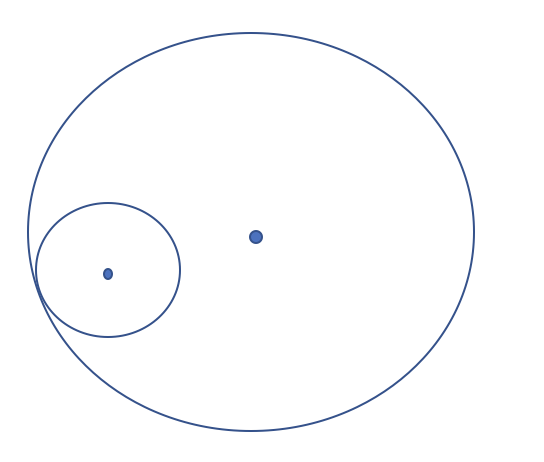
\includegraphics[width=4cm]{construction_of_contradictive_sequence}
\caption{The intuitive picture of construction of such a sequence}
\end{figure}
\paragraph{Excercise 1.5.3}$\Rightarrow$ To prove the boundeness, we already done it. The prove of closeness is the following. Because $Y$ is complete, a convergent sequence in $X$ that is Cauchy in $Y$ is convergent in $Y$. Simply put, the limit of a convergent sequence in $Y$ lies in $Y$. Therefore, it is closed.\\
$\Leftarrow$ By proposition 1.1.18, it is sufficient to only show the target statement with $(\mathbb{R}^n,d)$ be a sup norm metric. By theorem 9.1.14, for every sequence $a_{n}$ in $(\mathbb{R}^n,d)$, there exists a subsequence $b_{n1}$ that the sequence of first entry of each point in it is a convergent sequence.\\Use an instance to illustrate it this.\\
\[a_{n}=\{(1.1,1),(0,2),(1.01,3),(0,4),(1.001,5),\dots\} 
\]
\[b_{n1}=\{(1.1,1),(1.01,3),(1.001,5),\dots\}
\]
For the dimension of element in metric space $(\mathbb{R}^n,d)$ $n$ is a finite number, we can do similiar procedure --- find subsequence $b_{n2}$ of $b_{n1}$ --- on and on. Till we get $b_{nn}$ that every entry of it is convergent. Then obviously, for sup norm metric, $b_{nn}$ is convergent.$\Box$\\(Remark: hope you are not confused with the notation, the first n in $b_{nn}$ want to means it is a sequence instead a point, the second is used to index the sequence of those  sequences.---hopefully I didn't make it more confused)
\paragraph{Excercise1.5.7}
\begin{itemize}
\item[(a)]$\Rightarrow$ This has been proven before.\\
$\Leftarrow$ By definition, for any sequence in $Z$, there exists a convergent subsequence in $Y$ ($Y$ is compact). Also $Z$ is closed, the limit of this convergent sequence lies in $Z$.$\Box$
\end{itemize}

\paragraph{Excercise 1.5.8} All the statementd are trivial to prove. While it seems that there exists some further theories regarding this excercise.

\paragraph{Excercise 1.5.10} 
\begin{itemize}
\item[(a)]$X \subseteq B(x^{(1)},\varepsilon+d(x^{(1)},x^{(2)})+d(x^{(2)},x^{(3)})+\dots+d(x^{(n-1)},x^{(n)}))$
\item[(b)]\textcolor{red}{This question is tough. I haven't solved yet.} This is intuitive but hard to comprehend the hint.
\item[(c)]The big picture of the hint is clear.
\end{itemize}

\paragraph{Excercise 1.5.12}(b) When $X$ is finite, $(X,d)$ is compact. Else, it isn't.
\paragraph{Excercise 1.5.15} Assume $\cap_{\alpha\in I}K_{\alpha} = \varnothing$, then $X/\cap_{\alpha\in I}K_{\alpha}=X$. By Morgan's Law, we have $\cup_{\alpha\in I} X/K_{\alpha}=X$ $\dots$(1)\\
Because every $K_{\alpha}$ is closed, $X/K_{\alpha}$ is open. By (1) and compactness of $X$, we know that there exist finite subset $\cup(X/K_{\alpha})_{\alpha\in E}$ of $\cup(X/K_{\alpha})_{\alpha\in I}$ cover $X$. This implies a contradiction; a finite union $\cap(K_{\alpha})_{\alpha\in E}=\varnothing$.\\
Counterexample:\\$(Q,d)$ be the metric space. $K_{n}=\{x|x\in \mathbb{Q}, x\in[\sqrt{2}-\frac{1}{n},\sqrt{2}]\}$, as we can see, $\cup_{n\in\mathbb{N}}K_{n}=\varnothing$.

\begin{figure}[H]
\centering
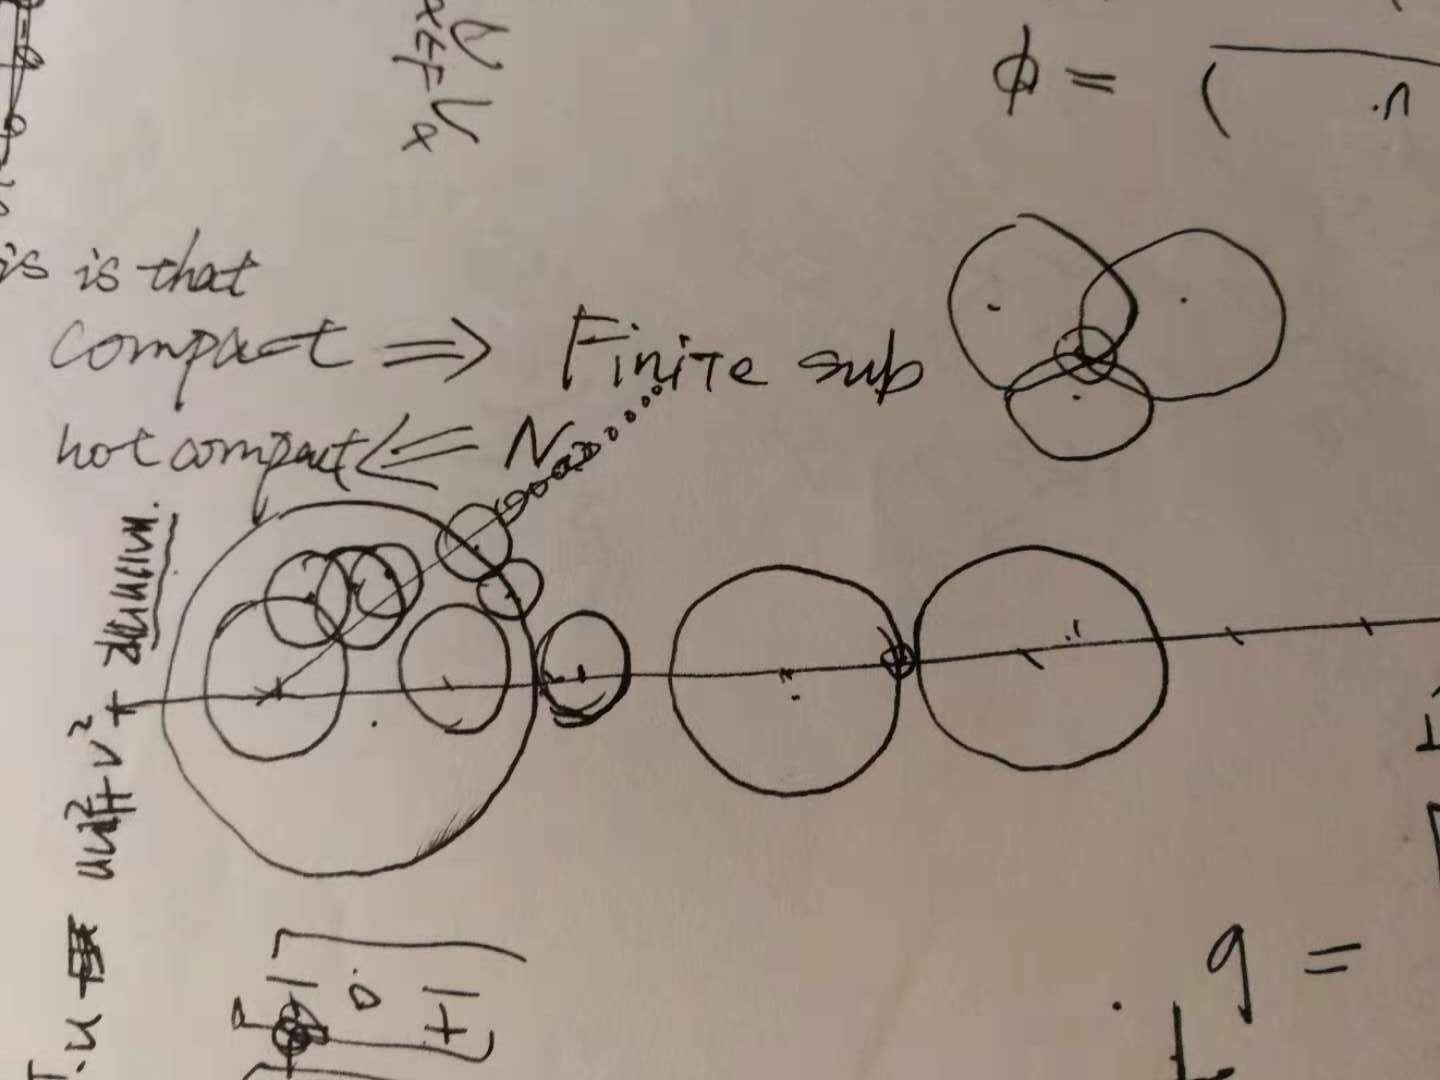
\includegraphics[width=6cm]{some_unspeakable_thoughts1.jpeg}
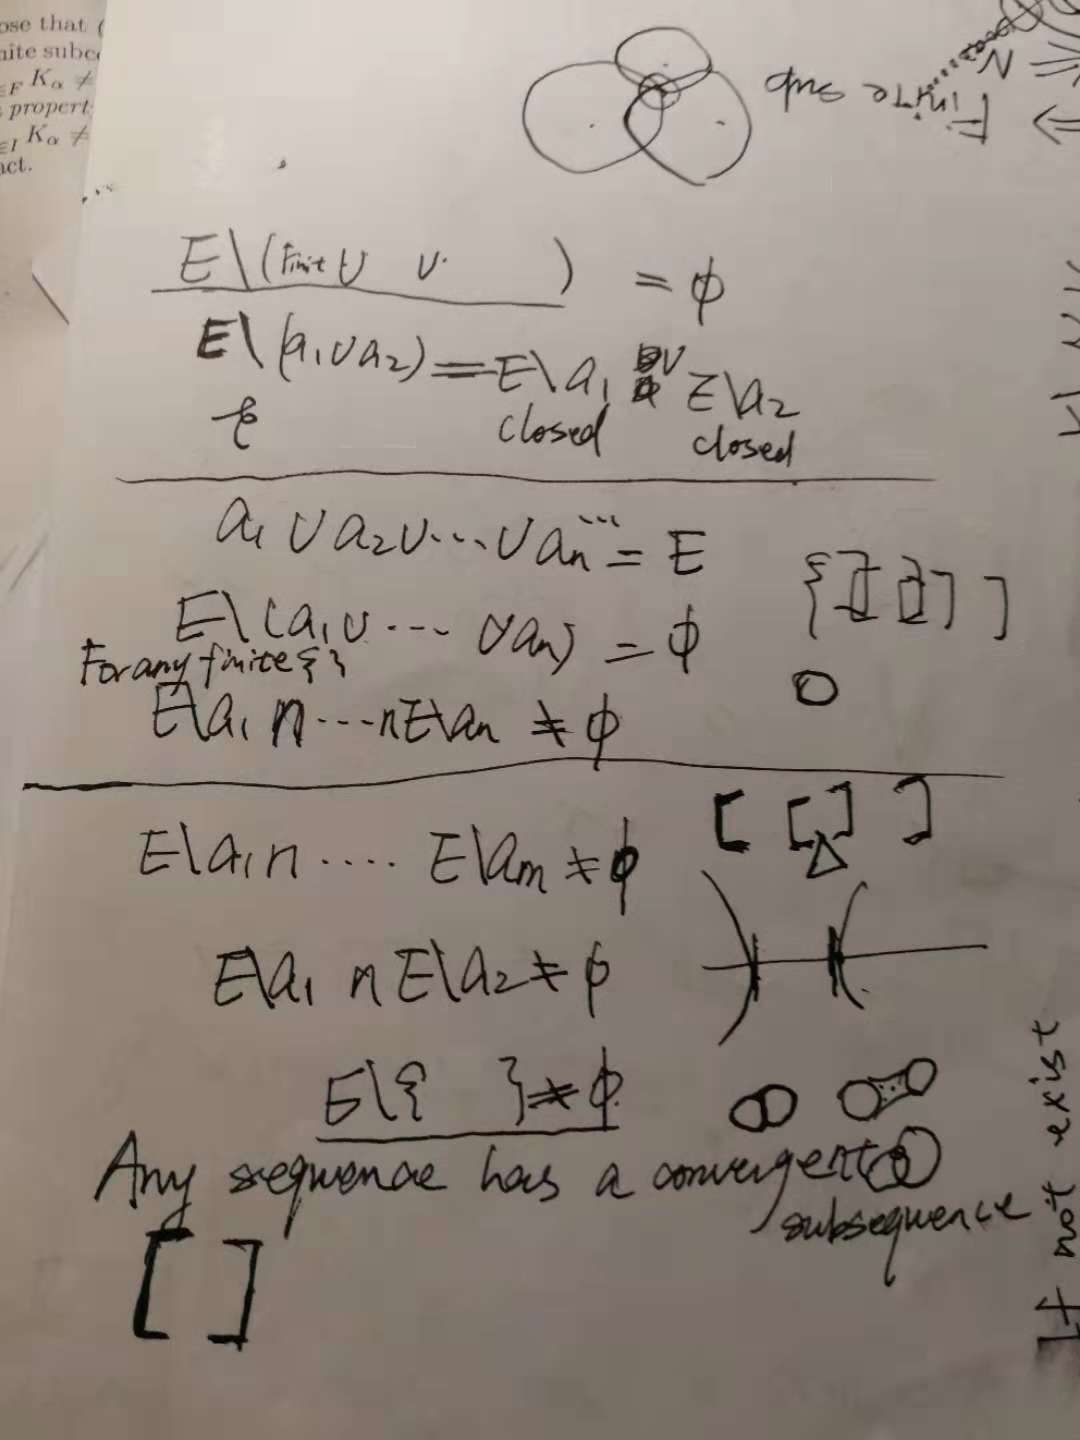
\includegraphics[width=6cm]{some_unspeakable_thoughts2.jpeg}
\caption{My primary thoughts before This excercise.}
\end{figure}





